% Options for packages loaded elsewhere
\PassOptionsToPackage{unicode}{hyperref}
\PassOptionsToPackage{hyphens}{url}
%
\documentclass[
  ignorenonframetext,
  aspectratio=169,
]{beamer}
\usepackage{pgfpages}
\setbeamertemplate{caption}[numbered]
\setbeamertemplate{caption label separator}{: }
\setbeamercolor{caption name}{fg=normal text.fg}
\beamertemplatenavigationsymbolsempty
% Prevent slide breaks in the middle of a paragraph
\widowpenalties 1 10000
\raggedbottom
\setbeamertemplate{part page}{
  \centering
  \begin{beamercolorbox}[sep=16pt,center]{part title}
    \usebeamerfont{part title}\insertpart\par
  \end{beamercolorbox}
}
\setbeamertemplate{section page}{
  \centering
  \begin{beamercolorbox}[sep=12pt,center]{part title}
    \usebeamerfont{section title}\insertsection\par
  \end{beamercolorbox}
}
\setbeamertemplate{subsection page}{
  \centering
  \begin{beamercolorbox}[sep=8pt,center]{part title}
    \usebeamerfont{subsection title}\insertsubsection\par
  \end{beamercolorbox}
}
\AtBeginPart{
  \frame{\partpage}
}
\AtBeginSection{
  \ifbibliography
  \else
    \frame{\sectionpage}
  \fi
}
\AtBeginSubsection{
  \frame{\subsectionpage}
}

\usepackage{amsmath,amssymb}
\usepackage{iftex}
\ifPDFTeX
  \usepackage[T1]{fontenc}
  \usepackage[utf8]{inputenc}
  \usepackage{textcomp} % provide euro and other symbols
\else % if luatex or xetex
  \usepackage{unicode-math}
  \defaultfontfeatures{Scale=MatchLowercase}
  \defaultfontfeatures[\rmfamily]{Ligatures=TeX,Scale=1}
\fi
\usepackage{lmodern}
\ifPDFTeX\else  
    % xetex/luatex font selection
  \setmonofont[Scale=0.35]{Menlo}
\fi
% Use upquote if available, for straight quotes in verbatim environments
\IfFileExists{upquote.sty}{\usepackage{upquote}}{}
\IfFileExists{microtype.sty}{% use microtype if available
  \usepackage[]{microtype}
  \UseMicrotypeSet[protrusion]{basicmath} % disable protrusion for tt fonts
}{}
\makeatletter
\@ifundefined{KOMAClassName}{% if non-KOMA class
  \IfFileExists{parskip.sty}{%
    \usepackage{parskip}
  }{% else
    \setlength{\parindent}{0pt}
    \setlength{\parskip}{6pt plus 2pt minus 1pt}}
}{% if KOMA class
  \KOMAoptions{parskip=half}}
\makeatother
\usepackage{xcolor}
\newif\ifbibliography
\setlength{\emergencystretch}{3em} % prevent overfull lines
\setcounter{secnumdepth}{-\maxdimen} % remove section numbering

\usepackage{color}
\usepackage{fancyvrb}
\newcommand{\VerbBar}{|}
\newcommand{\VERB}{\Verb[commandchars=\\\{\}]}
\DefineVerbatimEnvironment{Highlighting}{Verbatim}{commandchars=\\\{\}}
% Add ',fontsize=\small' for more characters per line
\usepackage{framed}
\definecolor{shadecolor}{RGB}{241,243,245}
\newenvironment{Shaded}{\begin{snugshade}}{\end{snugshade}}
\newcommand{\AlertTok}[1]{\textcolor[rgb]{0.68,0.00,0.00}{#1}}
\newcommand{\AnnotationTok}[1]{\textcolor[rgb]{0.37,0.37,0.37}{#1}}
\newcommand{\AttributeTok}[1]{\textcolor[rgb]{0.40,0.45,0.13}{#1}}
\newcommand{\BaseNTok}[1]{\textcolor[rgb]{0.68,0.00,0.00}{#1}}
\newcommand{\BuiltInTok}[1]{\textcolor[rgb]{0.00,0.23,0.31}{#1}}
\newcommand{\CharTok}[1]{\textcolor[rgb]{0.13,0.47,0.30}{#1}}
\newcommand{\CommentTok}[1]{\textcolor[rgb]{0.37,0.37,0.37}{#1}}
\newcommand{\CommentVarTok}[1]{\textcolor[rgb]{0.37,0.37,0.37}{\textit{#1}}}
\newcommand{\ConstantTok}[1]{\textcolor[rgb]{0.56,0.35,0.01}{#1}}
\newcommand{\ControlFlowTok}[1]{\textcolor[rgb]{0.00,0.23,0.31}{#1}}
\newcommand{\DataTypeTok}[1]{\textcolor[rgb]{0.68,0.00,0.00}{#1}}
\newcommand{\DecValTok}[1]{\textcolor[rgb]{0.68,0.00,0.00}{#1}}
\newcommand{\DocumentationTok}[1]{\textcolor[rgb]{0.37,0.37,0.37}{\textit{#1}}}
\newcommand{\ErrorTok}[1]{\textcolor[rgb]{0.68,0.00,0.00}{#1}}
\newcommand{\ExtensionTok}[1]{\textcolor[rgb]{0.00,0.23,0.31}{#1}}
\newcommand{\FloatTok}[1]{\textcolor[rgb]{0.68,0.00,0.00}{#1}}
\newcommand{\FunctionTok}[1]{\textcolor[rgb]{0.28,0.35,0.67}{#1}}
\newcommand{\ImportTok}[1]{\textcolor[rgb]{0.00,0.46,0.62}{#1}}
\newcommand{\InformationTok}[1]{\textcolor[rgb]{0.37,0.37,0.37}{#1}}
\newcommand{\KeywordTok}[1]{\textcolor[rgb]{0.00,0.23,0.31}{#1}}
\newcommand{\NormalTok}[1]{\textcolor[rgb]{0.00,0.23,0.31}{#1}}
\newcommand{\OperatorTok}[1]{\textcolor[rgb]{0.37,0.37,0.37}{#1}}
\newcommand{\OtherTok}[1]{\textcolor[rgb]{0.00,0.23,0.31}{#1}}
\newcommand{\PreprocessorTok}[1]{\textcolor[rgb]{0.68,0.00,0.00}{#1}}
\newcommand{\RegionMarkerTok}[1]{\textcolor[rgb]{0.00,0.23,0.31}{#1}}
\newcommand{\SpecialCharTok}[1]{\textcolor[rgb]{0.37,0.37,0.37}{#1}}
\newcommand{\SpecialStringTok}[1]{\textcolor[rgb]{0.13,0.47,0.30}{#1}}
\newcommand{\StringTok}[1]{\textcolor[rgb]{0.13,0.47,0.30}{#1}}
\newcommand{\VariableTok}[1]{\textcolor[rgb]{0.07,0.07,0.07}{#1}}
\newcommand{\VerbatimStringTok}[1]{\textcolor[rgb]{0.13,0.47,0.30}{#1}}
\newcommand{\WarningTok}[1]{\textcolor[rgb]{0.37,0.37,0.37}{\textit{#1}}}

\providecommand{\tightlist}{%
  \setlength{\itemsep}{0pt}\setlength{\parskip}{0pt}}\usepackage{longtable,booktabs,array}
\usepackage{calc} % for calculating minipage widths
\usepackage{caption}
% Make caption package work with longtable
\makeatletter
\def\fnum@table{\tablename~\thetable}
\makeatother
\usepackage{graphicx}
\makeatletter
\def\maxwidth{\ifdim\Gin@nat@width>\linewidth\linewidth\else\Gin@nat@width\fi}
\def\maxheight{\ifdim\Gin@nat@height>\textheight\textheight\else\Gin@nat@height\fi}
\makeatother
% Scale images if necessary, so that they will not overflow the page
% margins by default, and it is still possible to overwrite the defaults
% using explicit options in \includegraphics[width, height, ...]{}
\setkeys{Gin}{width=\maxwidth,height=\maxheight,keepaspectratio}
% Set default figure placement to htbp
\makeatletter
\def\fps@figure{htbp}
\makeatother

\makeatletter
\makeatother
\makeatletter
\makeatother
\makeatletter
\@ifpackageloaded{caption}{}{\usepackage{caption}}
\AtBeginDocument{%
\ifdefined\contentsname
  \renewcommand*\contentsname{Table of contents}
\else
  \newcommand\contentsname{Table of contents}
\fi
\ifdefined\listfigurename
  \renewcommand*\listfigurename{List of Figures}
\else
  \newcommand\listfigurename{List of Figures}
\fi
\ifdefined\listtablename
  \renewcommand*\listtablename{List of Tables}
\else
  \newcommand\listtablename{List of Tables}
\fi
\ifdefined\figurename
  \renewcommand*\figurename{Figure}
\else
  \newcommand\figurename{Figure}
\fi
\ifdefined\tablename
  \renewcommand*\tablename{Table}
\else
  \newcommand\tablename{Table}
\fi
}
\@ifpackageloaded{float}{}{\usepackage{float}}
\floatstyle{ruled}
\@ifundefined{c@chapter}{\newfloat{codelisting}{h}{lop}}{\newfloat{codelisting}{h}{lop}[chapter]}
\floatname{codelisting}{Listing}
\newcommand*\listoflistings{\listof{codelisting}{List of Listings}}
\makeatother
\makeatletter
\@ifpackageloaded{caption}{}{\usepackage{caption}}
\@ifpackageloaded{subcaption}{}{\usepackage{subcaption}}
\makeatother
\makeatletter
\@ifpackageloaded{tcolorbox}{}{\usepackage[skins,breakable]{tcolorbox}}
\makeatother
\makeatletter
\@ifundefined{shadecolor}{\definecolor{shadecolor}{rgb}{.97, .97, .97}}
\makeatother
\makeatletter
\makeatother
\makeatletter
\makeatother
\ifLuaTeX
  \usepackage{selnolig}  % disable illegal ligatures
\fi
\usepackage[]{natbib}
\bibliographystyle{plainnat}
\IfFileExists{bookmark.sty}{\usepackage{bookmark}}{\usepackage{hyperref}}
\IfFileExists{xurl.sty}{\usepackage{xurl}}{} % add URL line breaks if available
\urlstyle{same} % disable monospaced font for URLs
\hypersetup{
  pdftitle={ReSANGloW:},
  pdfauthor={Arturo Torres},
  hidelinks,
  pdfcreator={LaTeX via pandoc}}

\title{ReSANGloW:}
\subtitle{A Reproducible Spatial Analysis for Charting Nitrogen Dynamics
in Global Wheat Production}
\author{Arturo Torres}
\date{Wednesday, October 18, 2023}
\institute{LIST, ERIN}

\begin{document}
\frame{\titlepage}
\ifdefined\Shaded\renewenvironment{Shaded}{\begin{tcolorbox}[frame hidden, breakable, boxrule=0pt, interior hidden, sharp corners, borderline west={3pt}{0pt}{shadecolor}, enhanced]}{\end{tcolorbox}}\fi

\begin{frame}{Goal}
\protect\hypertarget{goal}{}
\begin{itemize}[<+->]
\item
  Following the indications, the goal of this reproducible code is to
  (IIASA-BNR, 2023, assignment):

  \begin{itemize}[<+->]
  \item
    ``Combine various datasets to generate indictors of nitrogen loss to
    the environment associated with wheat production at various spatial
    scales''
  \item
    ``Provide graphical representations and conduct simple comparisons
    across a few countries''
  \item
    ``Provide a reproducible code associated to these tasks.''
  \end{itemize}
\end{itemize}
\end{frame}

\begin{frame}{Task 1}
\protect\hypertarget{task-1}{}
\begin{itemize}[<+->]
\item
  Using SPAM raster data \citep{wood-sichra_spatial_2016}, a new raster
  at the same resolution, containing wheat production volume (in million
  tons Mt) is produced.
\item
  Global scale in a raster format (5 arcminute spatial resolution)
  estimates of yield in Kg/Ha, physical area in Ha and harvested area in
  Ha for the year 2005 are available.
\end{itemize}

\linespread{0.5}

\linespread{2}
\end{frame}

\begin{frame}[fragile]{Reading SPAM data}
\protect\hypertarget{reading-spam-data}{}
\linespread{0.5}

\begin{Shaded}
\begin{Highlighting}[]
\NormalTok{spam\_data }\OtherTok{=} \FunctionTok{list}\NormalTok{(}\StringTok{"yield"} \OtherTok{=} \FunctionTok{rast}\NormalTok{(}\StringTok{"data/SPAM\_2005\_v3.2/SPAM2005V3r2\_global\_Y\_TA\_WHEA\_A.tif"}\NormalTok{),}
                 \StringTok{"harvested\_area"} \OtherTok{=} \FunctionTok{rast}\NormalTok{(}\StringTok{"data/SPAM\_2005\_v3.2/SPAM2005V3r2\_global\_H\_TA\_WHEA\_A.tif"}\NormalTok{),}
                 \StringTok{"physical\_area"} \OtherTok{=} \FunctionTok{rast}\NormalTok{(}\StringTok{"data/SPAM\_2005\_v3.2/SPAM2005V3r2\_global\_A\_TA\_WHEA\_A.tif"}\NormalTok{))}
\end{Highlighting}
\end{Shaded}

\linespread{2}

\linespread{0.5}

\begin{Shaded}
\begin{Highlighting}[]
\FunctionTok{str}\NormalTok{(spam\_data)   }
\end{Highlighting}
\end{Shaded}

\begin{verbatim}
List of 3
 $ yield         :S4 class 'SpatRaster' [package "terra"]
 $ harvested_area:S4 class 'SpatRaster' [package "terra"]
 $ physical_area :S4 class 'SpatRaster' [package "terra"]
\end{verbatim}

\begin{Shaded}
\begin{Highlighting}[]
\NormalTok{spam\_data[[}\StringTok{\textquotesingle{}yield\textquotesingle{}}\NormalTok{]]}
\end{Highlighting}
\end{Shaded}

\begin{verbatim}
class       : SpatRaster 
dimensions  : 1853, 4320, 1  (nrow, ncol, nlyr)
resolution  : 0.08333333, 0.08333333  (x, y)
extent      : -180, 180, -64.41667, 90  (xmin, xmax, ymin, ymax)
coord. ref. : lon/lat WGS 84 (EPSG:4326) 
source      : SPAM2005V3r2_global_Y_TA_WHEA_A.tif 
name        : SPAM2005V3r2_global_Y_TA_WHEA_A 
min value   :                               0 
max value   :                           19429 
\end{verbatim}

\linespread{2}
\end{frame}

\begin{frame}{Calculate Wheat Production}
\protect\hypertarget{calculate-wheat-production}{}
\begin{itemize}[<+->]
\item
  Calculate wheat production by multiplying the raster layers for yield
  (in Kg/Ha) and harvested area (in Ha) using the * operator:

  \begin{itemize}[<+->]
  \tightlist
  \item
    wheat\_production = spam\_data{[}{[}``yield''{]}{]} *
    spam\_data{[}{[}``harvested\_area''{]}{]}
  \end{itemize}
\item
  Convert Units: The resulting values are in Kg, so it is needed to
  convert them to million tons (Mt). Assuming 1 ton is equal to 1,000
  Kg, it is possible to use the following:

  \begin{itemize}[<+->]
  \tightlist
  \item
    wheat\_production\_Mt = wheat\_production / (1e3 * 1e6)
  \end{itemize}
\end{itemize}
\end{frame}

\begin{frame}[fragile]{Calculate Wheat Production}
\protect\hypertarget{calculate-wheat-production-1}{}
\begin{itemize}[<+->]
\tightlist
\item
  A global map is created and the raster is exported in a geotif format:
\end{itemize}

\linespread{0.5}

\begin{Shaded}
\begin{Highlighting}[]
\NormalTok{wheat\_production }\OtherTok{=}\NormalTok{ spam\_data[[}\StringTok{"yield"}\NormalTok{]] }\SpecialCharTok{*}\NormalTok{ spam\_data[[}\StringTok{"harvested\_area"}\NormalTok{]]}
\NormalTok{wheat\_production\_Mt }\OtherTok{\textless{}{-}}\NormalTok{ wheat\_production }\SpecialCharTok{/}\NormalTok{ (}\FloatTok{1e9}\NormalTok{)}
\end{Highlighting}
\end{Shaded}

\linespread{2}

\linespread{0.5}

\begin{Shaded}
\begin{Highlighting}[]
\FunctionTok{library}\NormalTok{(raster)}

\FunctionTok{writeRaster}\NormalTok{(wheat\_production\_Mt, }\AttributeTok{filename =} \StringTok{"./output/wheat\_production\_Mt.tif"}\NormalTok{, }
            \AttributeTok{overwrite=}\ConstantTok{TRUE}\NormalTok{, }\AttributeTok{gdal =} \FunctionTok{c}\NormalTok{(}\StringTok{"COMPRESS=DEFLATE"}\NormalTok{, }\StringTok{"TFW=YES"}\NormalTok{))}
\end{Highlighting}
\end{Shaded}

\linespread{2}
\end{frame}

\begin{frame}{Wheat Production in Mt in 2005}
\protect\hypertarget{wheat-production-in-mt-in-2005}{}
\linespread{0.5}

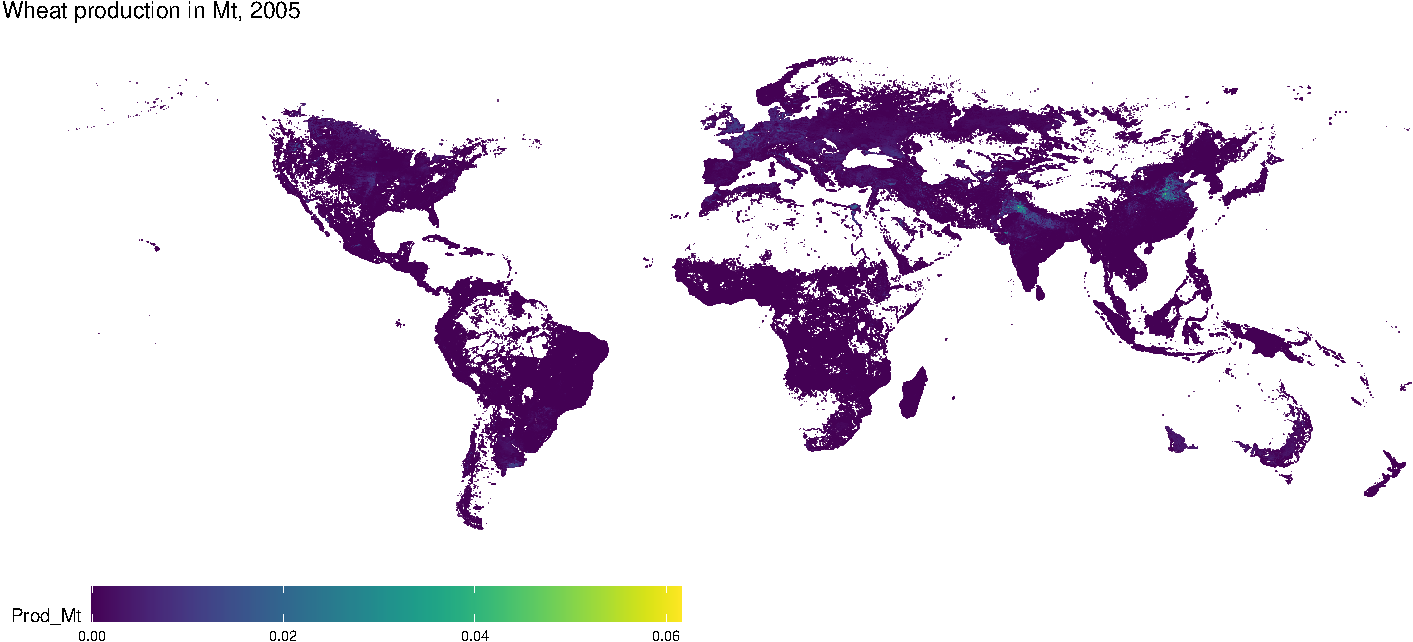
\includegraphics{global_n_files/figure-beamer/unnamed-chunk-7-1.pdf}

\linespread{2}
\end{frame}

\begin{frame}[fragile]{Task 2}
\protect\hypertarget{task-2}{}
\begin{itemize}[<+->]
\tightlist
\item
  Using the newly created raster and the GAUL shapefile of
  administrative borders, the production is aggregated to country level
  and exported to a csv file.
\end{itemize}

\linespread{0.5}

\begin{Shaded}
\begin{Highlighting}[]
\FunctionTok{library}\NormalTok{(raster)}
\FunctionTok{library}\NormalTok{(sf)}
\FunctionTok{library}\NormalTok{(rgdal)}
\FunctionTok{library}\NormalTok{(rgeos)}


\NormalTok{gaul\_data\_sf }\OtherTok{\textless{}{-}} \FunctionTok{st\_read}\NormalTok{(}\StringTok{"data/GAUL/g2015\_2005\_2.shp"}\NormalTok{)}
\end{Highlighting}
\end{Shaded}

\begin{verbatim}
Reading layer `g2015_2005_2' from data source 
  `/Users/torres/Documents/02_working/3-Production/05_models/32_iiasa/global_n/data/GAUL/g2015_2005_2.shp' 
  using driver `ESRI Shapefile'
Simple feature collection with 38189 features and 12 fields
Geometry type: MULTIPOLYGON
Dimension:     XY
Bounding box:  xmin: -180 ymin: -89.9 xmax: 180 ymax: 83.62742
Geodetic CRS:  WGS 84
\end{verbatim}

\begin{Shaded}
\begin{Highlighting}[]
\NormalTok{gaul\_data\_sp }\OtherTok{\textless{}{-}} \FunctionTok{readOGR}\NormalTok{(}\AttributeTok{dsn =} \StringTok{"./data/GAUL"}\NormalTok{, }\AttributeTok{layer =} \StringTok{"g2015\_2005\_2"}\NormalTok{)}
\end{Highlighting}
\end{Shaded}

\begin{verbatim}
OGR data source with driver: ESRI Shapefile 
Source: "/Users/torres/Documents/02_working/3-Production/05_models/32_iiasa/global_n/data/GAUL", layer: "g2015_2005_2"
with 38189 features
It has 12 fields
\end{verbatim}

\begin{Shaded}
\begin{Highlighting}[]
\NormalTok{gaul\_lev0 }\OtherTok{\textless{}{-}} \FunctionTok{levels}\NormalTok{(}\FunctionTok{factor}\NormalTok{(gaul\_data\_sp}\SpecialCharTok{@}\NormalTok{data[,}\StringTok{"ADM0\_NAME"}\NormalTok{]))}

\NormalTok{ids }\OtherTok{\textless{}{-}} \FunctionTok{lapply}\NormalTok{(gaul\_lev0, }\ControlFlowTok{function}\NormalTok{(x) }\FunctionTok{which}\NormalTok{(gaul\_data\_sp}\SpecialCharTok{@}\NormalTok{data[,}\StringTok{"ADM0\_NAME"}\NormalTok{] }\SpecialCharTok{==}\NormalTok{ x))}

\CommentTok{\# sp\_join \textless{}{-} as(gaul\_data\_sp, "SpatialPolygons")}
\end{Highlighting}
\end{Shaded}

\linespread{2}

\linespread{0.5}

\begin{Shaded}
\begin{Highlighting}[]
\ControlFlowTok{if}\NormalTok{(compute\_agg }\SpecialCharTok{==} \ConstantTok{TRUE}\NormalTok{) \{ }\DocumentationTok{\#\# Parallel computation}
  \FunctionTok{library}\NormalTok{(pbapply)}
  \FunctionTok{library}\NormalTok{(parallel)}
  \FunctionTok{library}\NormalTok{(doParallel)}
  
\NormalTok{  ncores }\OtherTok{=} \FunctionTok{detectCores}\NormalTok{() }\SpecialCharTok{{-}} \DecValTok{2}
  \CommentTok{\# ncores = 8}
\NormalTok{  cluster }\OtherTok{\textless{}{-}} \FunctionTok{makeCluster}\NormalTok{(ncores)}
  \FunctionTok{registerDoParallel}\NormalTok{(cluster, }\AttributeTok{cores=}\NormalTok{ncores)}
  
  \FunctionTok{clusterEvalQ}\NormalTok{(}\AttributeTok{cl =}\NormalTok{ cluster, }\FunctionTok{c}\NormalTok{(}\FunctionTok{library}\NormalTok{(rgeos, raster)))}
  \FunctionTok{clusterExport}\NormalTok{(}\AttributeTok{cl =}\NormalTok{ cluster, }\AttributeTok{varlist =} \FunctionTok{c}\NormalTok{(}\StringTok{"ids"}\NormalTok{, }\StringTok{"gaul\_data\_sp"}\NormalTok{))}
  
\NormalTok{  sp\_join\_lst }\OtherTok{\textless{}{-}} \FunctionTok{parLapply}\NormalTok{(}\AttributeTok{cl =}\NormalTok{ cluster, }\AttributeTok{X =} \DecValTok{1}\SpecialCharTok{:}\FunctionTok{length}\NormalTok{(ids), }\AttributeTok{fun =} \ControlFlowTok{function}\NormalTok{(i) \{}
    \FunctionTok{print}\NormalTok{(}\FunctionTok{paste0}\NormalTok{(i, }\StringTok{"/"}\NormalTok{, }\FunctionTok{length}\NormalTok{(ids)))}
    \FunctionTok{gUnionCascaded}\NormalTok{(gaul\_data\_sp[ids[[i]],])}
\NormalTok{  \})}

  \FunctionTok{stopCluster}\NormalTok{(}\AttributeTok{cl=}\NormalTok{cluster)}
  
  \FunctionTok{save}\NormalTok{(sp\_join\_lst, }\AttributeTok{file =} \StringTok{"./output/sp\_join\_lst.RData"}\NormalTok{)}
\NormalTok{\}}
\end{Highlighting}
\end{Shaded}

\linespread{2}

\linespread{0.5}

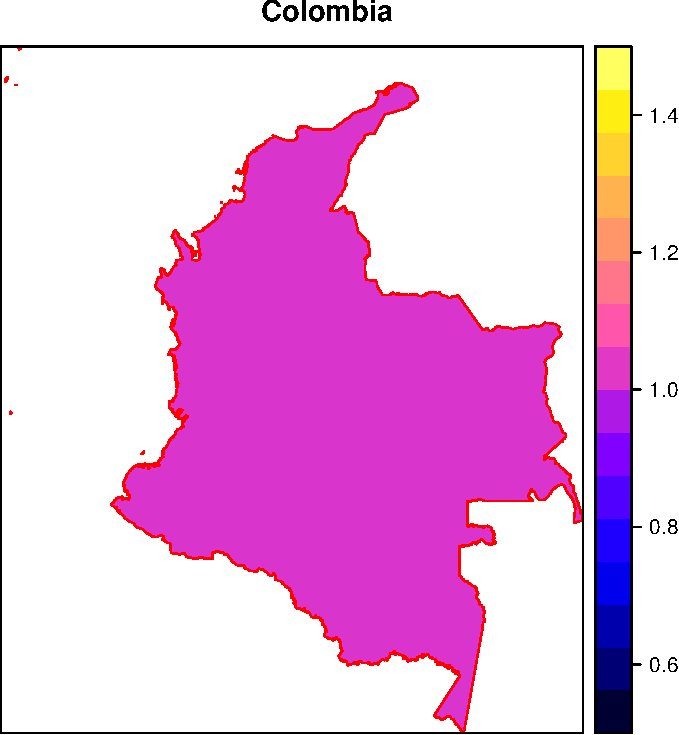
\includegraphics{global_n_files/figure-beamer/unnamed-chunk-8-1.pdf}

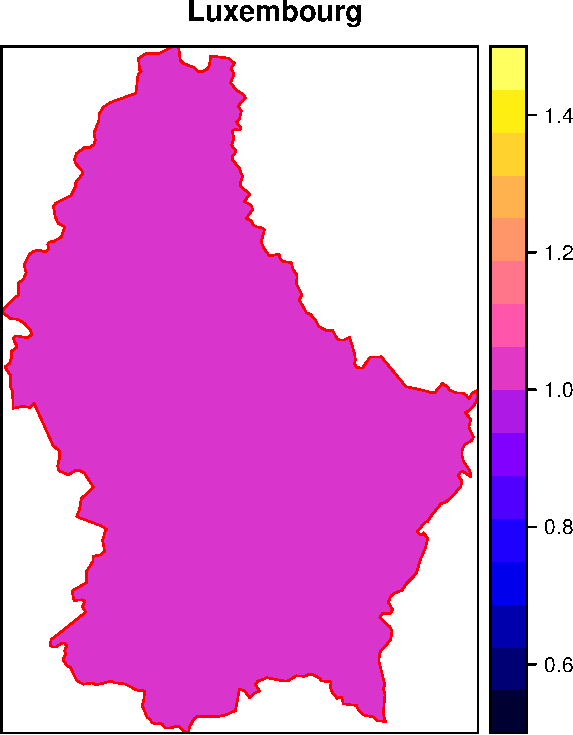
\includegraphics{global_n_files/figure-beamer/unnamed-chunk-8-2.pdf}

\linespread{2}

\linespread{0.5}

\linespread{2}

\linespread{0.5}

\linespread{2}

\linespread{0.5}

\linespread{2}
\end{frame}

\begin{frame}{Create a Data Frame and Rename Columns}
\protect\hypertarget{create-a-data-frame-and-rename-columns}{}
\begin{itemize}[<+->]
\item
  Rename the columns to indicate the country name and the aggregated
  wheat production in million tons.
\item
  The country\_production\_df contains a data frame with each country's
  name and its aggregated wheat production in million tons. This data
  frame can be used for further analysis or visualization, and export to
  a csv file.
\end{itemize}
\end{frame}

\begin{frame}[fragile]{Wheat Production: Top 10 Most Productive
Countries in 2005}
\protect\hypertarget{wheat-production-top-10-most-productive-countries-in-2005}{}
\linespread{0.5}

\begin{Shaded}
\begin{Highlighting}[]
\FunctionTok{load}\NormalTok{(}\StringTok{"./output/country\_aggregated\_production\_lst.RData"}\NormalTok{)}

\NormalTok{country\_production\_df }\OtherTok{=} \FunctionTok{data.frame}\NormalTok{(}\FunctionTok{do.call}\NormalTok{(}\AttributeTok{what =}\NormalTok{ rbind, }\AttributeTok{args =}\NormalTok{ country\_aggregated\_production\_lst)) }

\NormalTok{country\_production\_df}\SpecialCharTok{$}\NormalTok{ID }\OtherTok{=}\NormalTok{ gaul\_lev0}
\end{Highlighting}
\end{Shaded}

\linespread{2}

\linespread{0.5}

\begin{Shaded}
\begin{Highlighting}[]
\FunctionTok{colnames}\NormalTok{(country\_production\_df) }\OtherTok{\textless{}{-}} \FunctionTok{c}\NormalTok{( }\StringTok{"Country"}\NormalTok{, }\StringTok{"Wheat\_Production\_Mt"}\NormalTok{)}

\NormalTok{top10\_order }\OtherTok{=}\NormalTok{ country\_production\_df[}\FunctionTok{order}\NormalTok{(country\_production\_df}\SpecialCharTok{$}\NormalTok{Wheat\_Production\_Mt, }\AttributeTok{decreasing =} \ConstantTok{TRUE}\NormalTok{), ]}

\NormalTok{top10\_order[}\DecValTok{1}\SpecialCharTok{:}\DecValTok{10}\NormalTok{,]}
\end{Highlighting}
\end{Shaded}

\begin{verbatim}
                     Country Wheat_Production_Mt
52                     China            99.26530
117                    India            69.55773
260 United States of America            55.12679
206       Russian Federation            46.02241
85                    France            37.27257
46                    Canada            25.26367
93                   Germany            23.81824
189                 Pakistan            20.89733
251                   Turkey            20.83224
16                 Australia            19.30162
\end{verbatim}

\begin{Shaded}
\begin{Highlighting}[]
\FunctionTok{write.csv}\NormalTok{(country\_production\_df, }\AttributeTok{file =} \StringTok{"output/country\_production\_wheat.csv"}\NormalTok{)}
\end{Highlighting}
\end{Shaded}

\linespread{2}
\end{frame}

\begin{frame}[fragile]{Task 3}
\protect\hypertarget{task-3}{}
\begin{itemize}[<+->]
\item
  To create a raster map of the nitrogen (N) output in harvested wheat
  yield, assuming that 2\% of the harvested wheat yield consists of the
  N element, it is used again the ``raster'' package. Here are the steps
  to achieve this:

  \begin{itemize}[<+->]
  \item
    Read the ``wheat\_production'' raster created earlier in Task 1.
  \item
    Calculate Nitrogen Output Raster: A new raster that represents the
    nitrogen (N) output in harvested wheat yield is created. Assuming
    2\% of the harvested yield is N, the following formula is used:

    \begin{itemize}[<+->]
    \tightlist
    \item
      nitrogen\_output\_raster = wheat\_production\_raster * 0.02
    \end{itemize}
  \item
    Plot the Nitrogen Output Raster: Visualize the
    ``nitrogen\_output\_raster'' using the plot function from the
    ``raster'' package.
  \item
    Export the Nitrogen Output Raster: To export the raster map of
    nitrogen output, the writeRaster function is used and saved in
    GeoTiff format.
  \end{itemize}
\end{itemize}

\linespread{0.5}

\begin{Shaded}
\begin{Highlighting}[]
\FunctionTok{library}\NormalTok{(raster)}

\NormalTok{wheat\_production\_raster }\OtherTok{=} \FunctionTok{raster}\NormalTok{(}\StringTok{"output/wheat\_production\_Mt.tif"}\NormalTok{)}

\NormalTok{nitrogen\_output\_raster }\OtherTok{=}\NormalTok{ wheat\_production\_raster }\SpecialCharTok{*} \FloatTok{0.02}
\end{Highlighting}
\end{Shaded}

\linespread{2}
\end{frame}

\begin{frame}{Global Nitrogen Output}
\protect\hypertarget{global-nitrogen-output}{}
\begin{itemize}[<+->]
\tightlist
\item
  A raster map that represents the nitrogen (N) output in the harvested
  wheat yield has been created, based on the assumption that 2\% of the
  yield consists of the N element. This map will show the distribution
  of nitrogen output in million tons (Mt) across the Globe.
\end{itemize}
\end{frame}

\begin{frame}[fragile]{Global Nitrogen Output in Harvested Wheat Yield
in Mt in 2005}
\protect\hypertarget{global-nitrogen-output-in-harvested-wheat-yield-in-mt-in-2005}{}
\begin{columns}[T]
\begin{column}{0.95\textwidth}
\linespread{0.5}

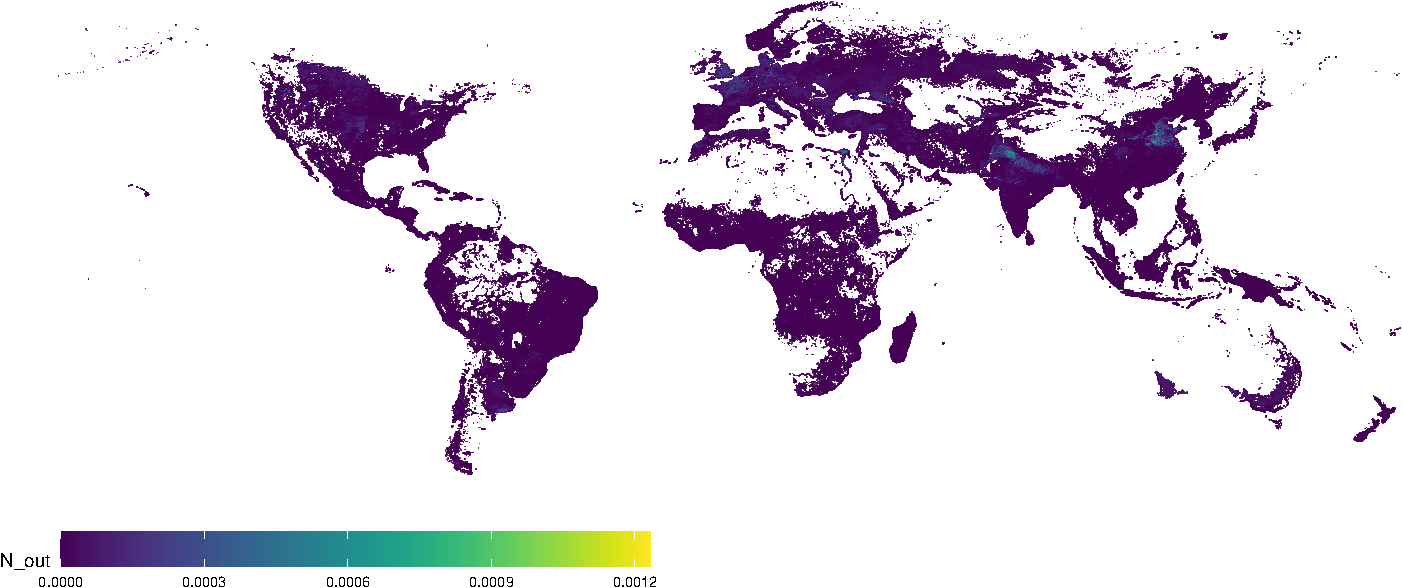
\includegraphics{global_n_files/figure-beamer/nitrogen-output-plot-1.pdf}

\linespread{2}
\end{column}
\end{columns}

\linespread{0.5}

\begin{Shaded}
\begin{Highlighting}[]
\NormalTok{raster}\SpecialCharTok{::}\FunctionTok{writeRaster}\NormalTok{(nitrogen\_output\_raster, }\AttributeTok{filename =} \StringTok{"output/nitrogen\_output.tif"}\NormalTok{, }\AttributeTok{format =} \StringTok{"GTiff"}\NormalTok{, }\AttributeTok{overwrite =} \ConstantTok{TRUE}\NormalTok{)}
\end{Highlighting}
\end{Shaded}

\linespread{2}
\end{frame}

\begin{frame}{Task 4}
\protect\hypertarget{task-4}{}
\begin{itemize}[<+->]
\item
  Using the dataset of country-level nitrogen use efficiency (NUE) of
  wheat from \citep{zhang_managing_2015}, and steps from previous tasks:

  \begin{itemize}[<+->]
  \item
    \begin{enumerate}[<+->]
    [a.]
    \tightlist
    \item
      For the 10 biggest wheat producers the country-level values of N
      output in harvested wheat, as well as related total N inputs and N
      losses (i.e., surplus) is estimated, and exported the dataset as a
      csv file
    \end{enumerate}
  \item
    \begin{enumerate}[<+->]
    [a.]
    \setcounter{enumi}{1}
    \tightlist
    \item
      The N outputs and losses for these 10 countries are summarized in
      one figure (plot exported as pdf file)
    \end{enumerate}
  \end{itemize}
\end{itemize}
\end{frame}

\begin{frame}[fragile]{a. Estimated and Exported Dataset for the Top 10
Countries by N Outputs and Losses}
\protect\hypertarget{a.-estimated-and-exported-dataset-for-the-top-10-countries-by-n-outputs-and-losses}{}
\linespread{0.5}

\linespread{2}

\linespread{0.5}

\linespread{2}

\linespread{0.5}

\begin{verbatim}
    NUE.Country NUE.NUE Production_Mt N_Output_Mt N_Inputs_Mt N_Losses_Mt
6         China    0.26         99.27        1.99       26.04       24.06
19        India    0.25         69.56        1.39       17.38       15.99
106         USA    0.51         55.13        1.10       28.00       26.90
75   RussianFed    0.62         46.02        0.92       28.48       27.56
7        France    0.74         37.27        0.75       27.65       26.91
5        Canada    0.50         25.26        0.51       12.72       12.21
8       Germany    0.46         23.82        0.48       10.92       10.45
65     Pakistan    0.20         20.90        0.42        4.18        3.76
99       Turkey    0.42         20.83        0.42        8.80        8.39
2     Australia    0.54         19.30        0.39       10.44       10.05
\end{verbatim}

\linespread{2}
\end{frame}

\begin{frame}{b. Visualization of the N Outputs and Losses}
\protect\hypertarget{b.-visualization-of-the-n-outputs-and-losses}{}
\linespread{0.5}

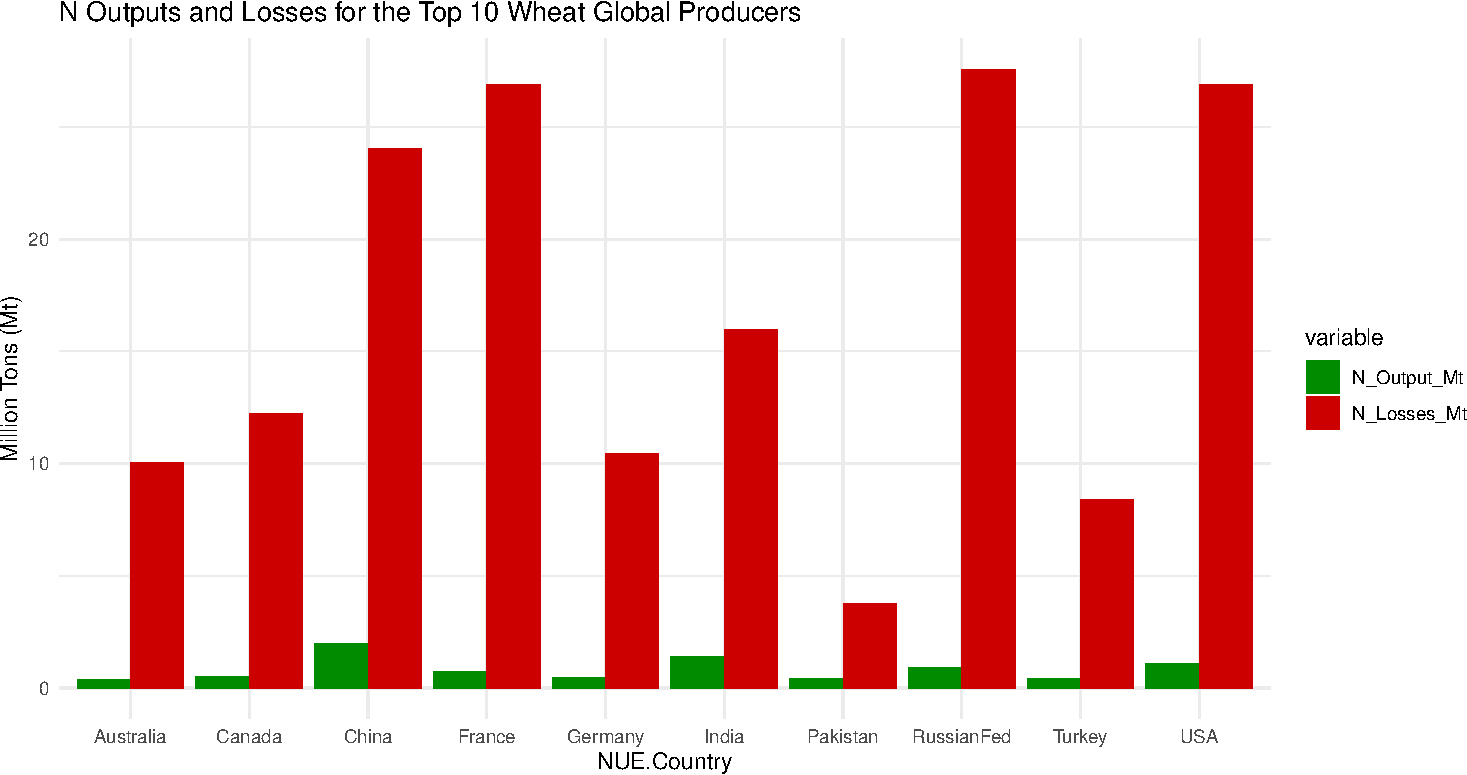
\includegraphics{global_n_files/figure-beamer/unnamed-chunk-15-1.pdf}

\linespread{2}
\end{frame}

\begin{frame}{c.~Main Patterns of N Lossess across Countries}
\protect\hypertarget{c.-main-patterns-of-n-lossess-across-countries}{}
\begin{itemize}[<+->]
\item
  The main patterns of N losses across countries, in relation to
  production volume and NUE (including any singular feature) are
  explained in the following paragraph:

  \begin{itemize}[<+->]
  \tightlist
  \item
    In the analysis of the top 10 wheat-producing countries, varying
    patterns of nitrogen losses is observed. Some countries with high
    wheat production volumes and relatively low NUE, such as China,
    showed significant nitrogen losses, suggesting inefficiencies in
    nitrogen utilization. In contrast, countries with relative higher
    NUE, like Australia, exhibited lower losses despite high production.
    Additionally, a few countries, like France, displayed unexpected
    patterns of high losses compared to their NUE, potentially
    indicating other factors influencing nitrogen loss, such as
    agricultural practices or environmental conditions.
  \end{itemize}
\end{itemize}
\end{frame}

\begin{frame}{Task 5}
\protect\hypertarget{task-5}{}
In the following paragraph is explained how an analysis like the one
performed in previous tasks could translate to the models within BNR's
modeling suite (https://iiasa.github.io/iBIOM/en/main/), including
potential limitations.

\begin{itemize}[<+->]
\tightlist
\item
  An analysis of nitrogen output, inputs, and losses in wheat production
  can inform IIASA BNR's modeling suite by providing critical data
  inputs for assessing the environmental impacts of agricultural
  practices. These data help in calibrating and validating models
  related to land use, nutrient management, and climate change
  mitigation, enhancing the suite's accuracy in predicting the effects
  of different agricultural scenarios on nitrogen cycling and
  environmental sustainability. Limitations, however, may arise from the
  simplifications made e.g.~in assuming a fixed 2\% nitrogen content in
  harvested yield, as actual values can vary. Additionally, model
  outcomes depend on the quality and comprehensiveness of input data,
  which can pose challenges in areas with limited data availability.
\end{itemize}
\end{frame}

\begin{frame}{Task 6}
\protect\hypertarget{task-6}{}
\begin{block}{Issues}
\protect\hypertarget{issues}{}
\begin{itemize}[<+->]
\item
  In the Task 2, an implementation of the country-level aggregation step
  for computing the Global wheat production per country in parallel was
  needed due to the high computational burden reached and avoid RAM
  issues. Therefore, parallel pre-computed RData objects were created to
  be loaded in this step to render this reproducible presentation in a
  reasonable short time (less than one minute), i.e.

  \begin{itemize}[<+->]
  \item
    ``./output/sp\_join\_lst.RData''
  \item
    ``./output/raster\_lst.RData''
  \item
    ``./output/country\_aggregated\_production\_lst.RData''
  \end{itemize}
\item
  Similarly in Task 3 the actual computation of the Global country
  production was coded in parallel and saved as an RData object to be
  loaded subsequently, i.e.

  \begin{itemize}[<+->]
  \tightlist
  \item
    ``./output/country\_aggregated\_N\_lst.RData''
  \end{itemize}
\end{itemize}
\end{block}
\end{frame}

\begin{frame}{Task 6}
\protect\hypertarget{task-6-1}{}
\begin{block}{Assumptions}
\protect\hypertarget{assumptions}{}
\begin{itemize}[<+->]
\item
  The computations were done by using the Geodetic CRS: WGS 84.
\item
  The three input maps from the SPAM model for the year 2005 are global
  scale in raster format (5 arcminute spatial resolution):

  \begin{itemize}[<+->]
  \tightlist
  \item
    Estimates of yield in Kg/Ha,
  \item
    Physical area in Ha,
  \item
    Harvested area in Ha.
  \end{itemize}
\item
  1 ton is equal to 1,000 Kg, so 1 million ton is equal to 1,000,000,000
  Kg, i.e.~1 million ton = 1e9 Kg.
\end{itemize}
\end{block}
\end{frame}

\begin{frame}{References}
\protect\hypertarget{references}{}
\renewcommand{\bibsection}{}
\bibliography{global_n.bib}
\end{frame}

\begin{frame}[fragile]{Session Info}
\protect\hypertarget{session-info}{}
\linespread{0.5}

\begin{verbatim}
Time difference of 36.1796 secs
\end{verbatim}

\linespread{2}

\linespread{0.5}

\begin{verbatim}
- Session info ---------------------------------------------------------------
 setting  value
 version  R version 4.2.0 (2022-04-22)
 os       macOS 13.4.1
 system   aarch64, darwin20
 ui       X11
 language (EN)
 collate  en_US.UTF-8
 ctype    en_US.UTF-8
 tz       Europe/Luxembourg
 date     2023-10-18
 pandoc   3.1.6.2 @ /opt/homebrew/bin/ (via rmarkdown)

- Packages -------------------------------------------------------------------
 package     * version date (UTC) lib source
 class         7.3-21  2023-01-23 [2] CRAN (R 4.2.0)
 classInt      0.4-9   2023-02-28 [1] CRAN (R 4.2.0)
 cli           3.6.0   2023-01-09 [1] CRAN (R 4.2.0)
 codetools     0.2-19  2023-02-01 [2] CRAN (R 4.2.0)
 colorspace    2.1-0   2023-01-23 [1] CRAN (R 4.2.0)
 DBI           1.1.3   2022-06-18 [1] CRAN (R 4.2.0)
 digest        0.6.31  2022-12-11 [1] CRAN (R 4.2.0)
 dplyr         1.1.3   2023-09-03 [1] CRAN (R 4.2.0)
 e1071         1.7-13  2023-02-01 [1] CRAN (R 4.2.0)
 evaluate      0.20    2023-01-17 [1] CRAN (R 4.2.0)
 fansi         1.0.4   2023-01-22 [1] CRAN (R 4.2.0)
 farver        2.1.1   2022-07-06 [1] CRAN (R 4.2.0)
 fastmap       1.1.1   2023-02-24 [1] CRAN (R 4.2.0)
 generics      0.1.3   2022-07-05 [1] CRAN (R 4.2.0)
 ggplot2     * 3.4.1   2023-02-10 [1] CRAN (R 4.2.0)
 ggthemes    * 4.2.4   2021-01-20 [1] CRAN (R 4.2.0)
 glue          1.6.2   2022-02-24 [1] CRAN (R 4.2.0)
 gridExtra     2.3     2017-09-09 [1] CRAN (R 4.2.0)
 gtable        0.3.1   2022-09-01 [1] CRAN (R 4.2.0)
 htmltools     0.5.4   2022-12-07 [1] CRAN (R 4.2.0)
 jsonlite      1.8.4   2022-12-06 [1] CRAN (R 4.2.0)
 KernSmooth    2.23-20 2021-05-03 [2] CRAN (R 4.2.0)
 knitr         1.42    2023-01-25 [1] CRAN (R 4.2.0)
 labeling      0.4.2   2020-10-20 [1] CRAN (R 4.2.0)
 lattice       0.20-45 2021-09-22 [2] CRAN (R 4.2.0)
 lifecycle     1.0.3   2022-10-07 [1] CRAN (R 4.2.0)
 magrittr      2.0.3   2022-03-30 [1] CRAN (R 4.2.0)
 munsell       0.5.0   2018-06-12 [1] CRAN (R 4.2.0)
 pillar        1.9.0   2023-03-22 [1] CRAN (R 4.2.0)
 pkgconfig     2.0.3   2019-09-22 [1] CRAN (R 4.2.0)
 plyr          1.8.8   2022-11-11 [1] CRAN (R 4.2.0)
 proxy         0.4-27  2022-06-09 [1] CRAN (R 4.2.0)
 purrr         1.0.1   2023-01-10 [1] CRAN (R 4.2.0)
 R6            2.5.1   2021-08-19 [1] CRAN (R 4.2.0)
 ragg          1.2.5   2023-01-12 [1] CRAN (R 4.2.0)
 raster      * 3.6-20  2023-03-06 [1] CRAN (R 4.2.0)
 Rcpp          1.0.10  2023-01-22 [1] CRAN (R 4.2.0)
 reshape2    * 1.4.4   2020-04-09 [1] CRAN (R 4.2.0)
 rgdal       * 1.6-5   2023-03-02 [1] CRAN (R 4.2.0)
 rgeos       * 0.6-2   2023-03-02 [1] CRAN (R 4.2.0)
 rlang         1.1.1   2023-04-28 [1] CRAN (R 4.2.0)
 rmarkdown     2.20    2023-01-19 [1] CRAN (R 4.2.0)
 rstudioapi    0.14    2022-08-22 [1] CRAN (R 4.2.0)
 scales      * 1.2.1   2022-08-20 [1] CRAN (R 4.2.0)
 sessioninfo * 1.2.2   2021-12-06 [1] CRAN (R 4.2.0)
 sf          * 1.0-9   2022-11-08 [1] CRAN (R 4.2.0)
 sp          * 1.6-0   2023-01-19 [1] CRAN (R 4.2.0)
 stringi       1.7.12  2023-01-11 [1] CRAN (R 4.2.0)
 stringr       1.5.0   2022-12-02 [1] CRAN (R 4.2.0)
 systemfonts   1.0.4   2022-02-11 [1] CRAN (R 4.2.0)
 terra       * 1.7-18  2023-03-06 [1] CRAN (R 4.2.0)
 textshaping   0.3.6   2021-10-13 [1] CRAN (R 4.2.0)
 tibble        3.2.1   2023-03-20 [1] CRAN (R 4.2.0)
 tidyselect    1.2.0   2022-10-10 [1] CRAN (R 4.2.0)
 units         0.8-1   2022-12-10 [1] CRAN (R 4.2.0)
 utf8          1.2.3   2023-01-31 [1] CRAN (R 4.2.0)
 vctrs         0.6.4   2023-10-12 [1] CRAN (R 4.2.0)
 viridis     * 0.6.2   2021-10-13 [1] CRAN (R 4.2.0)
 viridisLite * 0.4.1   2022-08-22 [1] CRAN (R 4.2.0)
 withr         2.5.0   2022-03-03 [1] CRAN (R 4.2.0)
 xfun          0.37    2023-01-31 [1] CRAN (R 4.2.0)
 yaml          2.3.7   2023-01-23 [1] CRAN (R 4.2.0)

 [1] /Users/torres/Library/R/arm64/4.2/library
 [2] /Library/Frameworks/R.framework/Versions/4.2-arm64/Resources/library

- External software ----------------------------------------------------------
 setting        value
 cairo          1.16.0
 cairoFT        2.11.1/2.13.94
 pango
 png            1.6.37
 jpeg           9.4
 tiff           LIBTIFF, Version 4.3.0
 tcl            8.6.12
 curl           7.88.1
 zlib           1.2.11
 bzlib          1.0.8, 13-Jul-2019
 xz             5.2.5
 PCRE           10.39 2021-10-29
 ICU            70.2
 TRE            TRE 0.8.0 R_fixes (BSD)
 iconv          GNU libiconv 1.11
 readline       5.2
 BLAS           /Library/Frameworks/R.framework/Versions/4.2-arm64/Resources/lib/libRblas.0.dylib
 lapack         /Library/Frameworks/R.framework/Versions/4.2-arm64/Resources/lib/libRlapack.dylib
 lapack_version 3.10.0

- Python configuration -------------------------------------------------------
 Python is not available

------------------------------------------------------------------------------
\end{verbatim}

\linespread{2}
\end{frame}


\begin{frame}[allowframebreaks]{}
  \bibliographytrue
\end{frame}


\end{document}
